\documentclass[12pt,letterpaper]{ntdhw}


\usepackage{ntdmath}

\title{Project 1: Regular Languages and Pursuit-Evasion}
\author{CSCI 561}

\rhead{Names: Shadi Nourriz, Nathaniel Graves, Rhett Houston}

%\keytrue

\begin{document}
\pagestyle{fancyplain}

\maketitle
\thispagestyle{fancyplain}
%\clearpage

\section*{Application: Text Processing with Grep}

\begin{quote}
  \emph{\texttt{grep} is a unix utility that searches text for lines
    matching a regular expression.}
\end{quote}

\begin{enumerate}
  \item \textbf{Using Grep:} Use the standard unix (or GNU)
  \texttt{grep} and the implementation in this project to search the
  starter code for all \texttt{TODO}s.

  \begin{figure}[h!]
    \centering
    \begin{minipage}{0.45\textwidth}
        \centering
        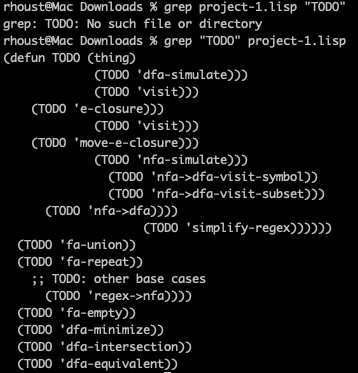
\includegraphics[width=0.9\textwidth]{grepScreenCap.png}
        \caption{Searching for Project \texttt{TODO}s using \texttt{grep}}
    \end{minipage}\hfill
    \begin{minipage}{0.55\textwidth}
        \centering
        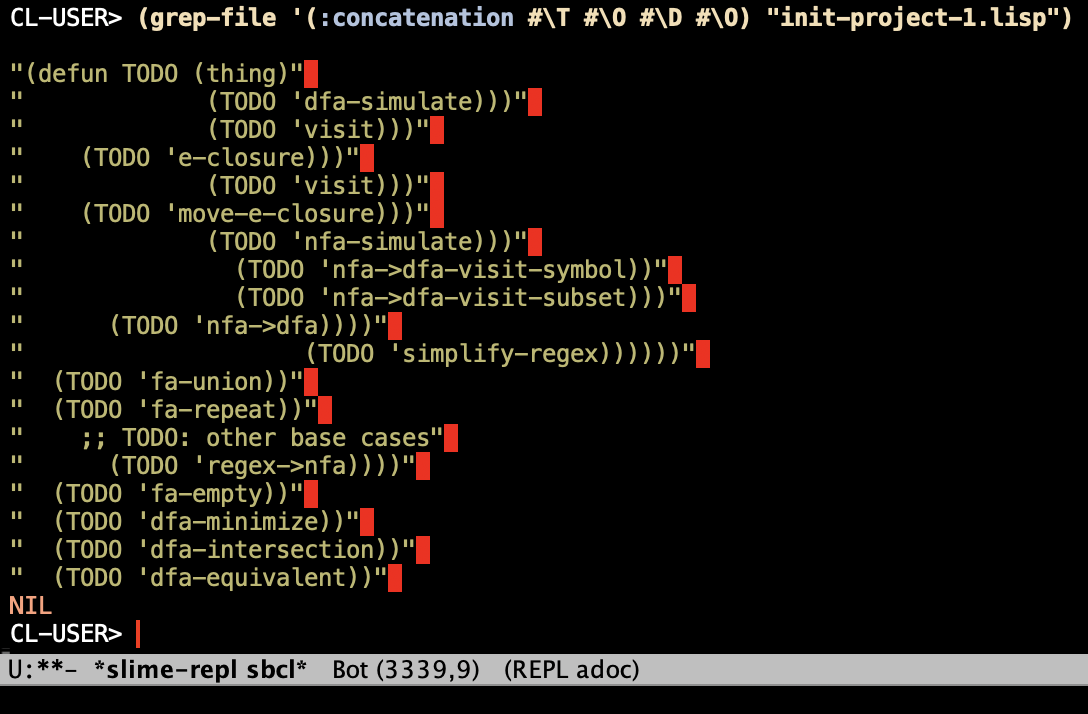
\includegraphics[width=1.0\textwidth]{1_project.png}
        \caption{Using \texttt{grep-file}}
    \end{minipage}
  \end{figure}

  \item \textbf{NFA vs. DFA Simulation:} The original grep utility (as
  written by Ken Thompson) converted the provided regular expression
  to an NFA and then simulated the NFA on the input text.  Why would
  Thompson have used NFA simulation instead of DFA simulation?

  \smallskip

  Thompson used direct NFA simulation because the alternative would mean he would need to convert the provided regular expression to an NFA, then a DFA. The conversion from NFA to DFA is an expensive one, from a time and space perspective. For small inputs, using direct NFA simulation makes more sense because it will likely have better time complexity than conversion to a DFA and then DFA simulation. For large inputs, the conversion from NFA to DFA could produce exponential numbers of states, which would use too much memory (poor space-complexity). 

  In short, Thompson used direct NFA simulation because it has better time and space complexity for small and large inputs, respectively.

  \clearpage

  \item \textbf{Time Complexity:} To simulate an NFA
  $N=\lmtuple{Q}{\Sigma}{\delta}{q_0}{F}$ on string $\sigma$ using the
  algorithm in the original grep (which is roughly equivalent to the
  NFA simulation algorithm covered in lecture) requires
  $O(|Q|*|\sigma|)$ time. However, many ``regex'' engines (including the
  popular implementation in Perl) exhibit worst-case complexity that
  is exponential in $|\sigma|$.

  \begin{enumerate}
    \item Prove that NFA simulation is possible in $O(|Q|*|\sigma|)$
    time.%

    \smallskip

    \begin{itemize}
        \item To prove NFA simulation possible in $O(|Q| * |\sigma|)$ time, we will use a proof by construction.
        \item Looking at the algorithm explained in lecture, we arrive at a few steps:
        \begin{enumerate}
            \item Take, as input, the NFA itself and an input sequence. 
            \item Let $q_0$ be the set of start states and let $F$ be the set of accepting states.
            \item Perform e-closure on $q_0$.
            \item Then, iterate through the elements of the input sequence, and use the current iteration's element in the call to e-closure. Save the new set of states arrived at, $q_i$, every time an iteration occurs. 
            \item Continue until e-closure does not return any more states or all the input sequence's elements have been followed. 
            \item If the final version of $(q_i \in F)$, then we accept. 
        \end{enumerate}
        \item Looking at step v., we can see that the algorithm ends after either all of the states, $Q$, have been visited, or, after the input sequence runs out of elements to be followed. 
        \item In the case that an input sequence requires both all states to be visited and iterates through all elements of an input sequence, the algorithm will take, at the most, $O(|Q| * |\sigma|)$ time.
        \item We have proven that NFA simulation is possible within $O(|Q| * |\sigma|)$ time. $\square$
    \end{itemize}

    \medskip

    \item Why is there such a difference in performance between
    Thompson's grep and some other ``regex'' engines?

    \smallskip
    
    There is a difference in performance between Thompson's grep and other ``regex'' engines because other regex engines may convert their NFAs to DFAs before simulating - whereas Thompson simulates NFAs directly. As alluded to in question 2, the conversion from NFA to DFA may sometimes result in DFAs with exponentially more states than the NFA originally had - meaning the conversion, from NFA to DFA, can prove very costly at times - in the worst case, exponential in $|\sigma|$.
    
  \end{enumerate}

\end{enumerate}

\clearpage

\section*{Application: Discrete Event Systems Model of Pursuit-Evasion}

\begin{quote}

\emph{\emph{Pursuit-evasion games} are scenarios with multiple agents
  where one agent attempts to avoid capture by another.  Consider a
  variation of pursuit-evasion games as follows:}

\begin{itemize}
  \item \it Two agents share a grid environment: a human (evader) and wumpus
  (pursuer).
  \item \it The human and wumpus alternate moves on the grid.  The
  wumpus moves each turn up, down, left or right.  The human can move
  up, down, left, right, or remain in place.  You may assume that the
  human moves first.
  \item \it If the wumpus and human ever occupy the same grid cell,
  the wumpus eats the human.
  \item \it If the human reaches a designated grid cell, they escape.
\end{itemize}

\emph{Answer the following questions using your implementation of finite
automata operations for support.}

\end{quote}

\begin{figure}[ht]
  \centering
  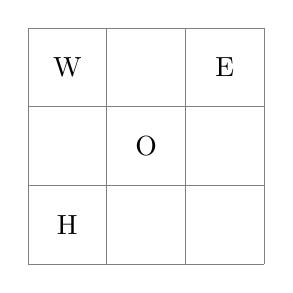
\begin{tikzpicture}
    \draw[step=1cm,gray,very thin,xshift=.5cm,yshift=.5cm] (-1,-1) grid (2,2);
    \node at (0cm,2cm) {W};
    \node at (0cm,0cm) {H};
    \node at (1cm,1cm) {O};
    \node at (2cm,2cm) {E};
  \end{tikzpicture}
  \caption{Example wumpus-world map.  W represents the initial
    location of the wumpus.  H represents the initial location of the
    human.  E represents the escape location.  O represents an
    obstacle that neither the human nor wumpus can move into.}
  \label{fig:map}
\end{figure}

\begin{enumerate}

  \item For the map in \ref{fig:map}, construct a discrete event
  system model.  Assume that the human's movements are controllable
  and that the wumpus's movements are not controllable.

  \begin{figure}[ht]
      \centering
      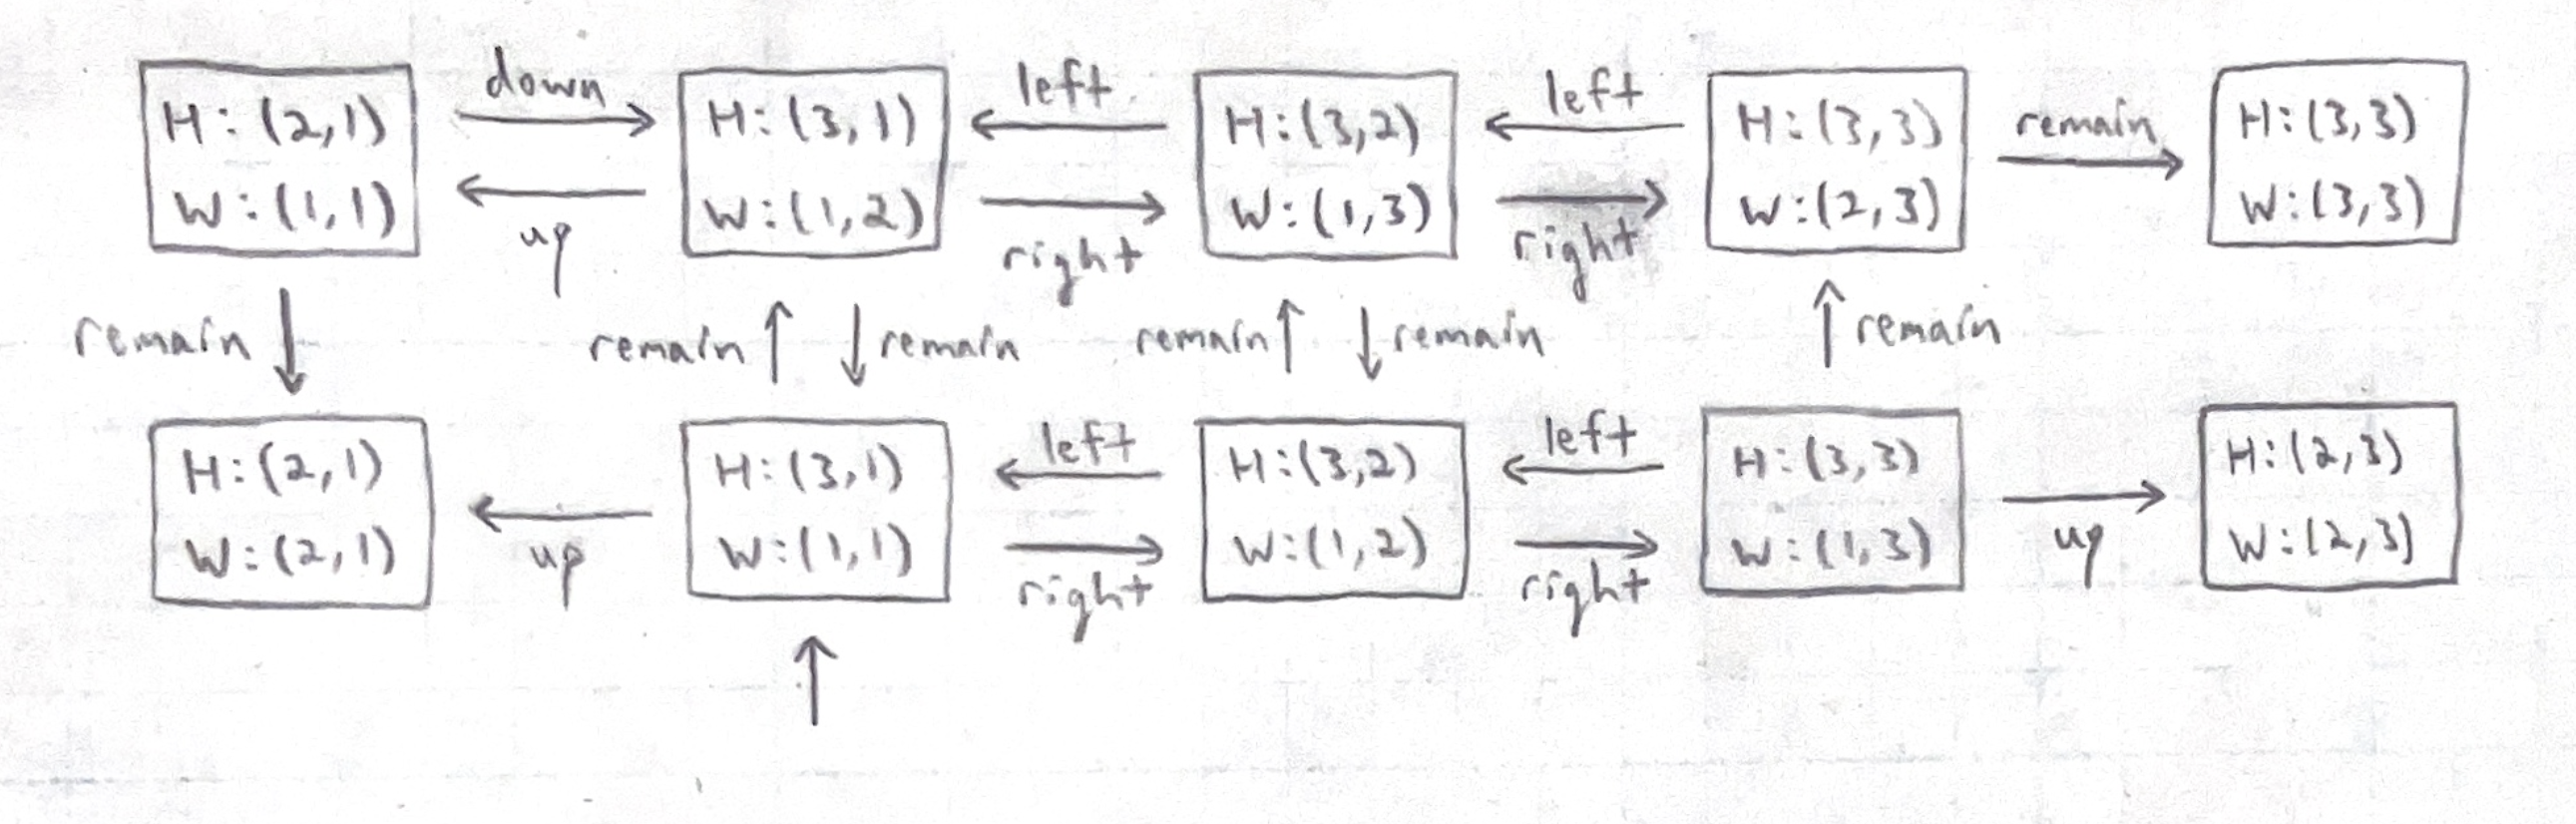
\includegraphics[width=0.9\textwidth]{2_human.png}
  \end{figure}

\clearpage

  \item For your DES model of \ref{fig:map}, construct a specification
  for the human to avoid the wumpus and escape.
  \begin{enumerate}
    \item Can the human guarantee to avoid being eaten, no matter what
    the wumpus does?  Prove yes or no via automata operations.
    \item Can the human always escape in finite time (fixed
    number of steps), no matter what the wumpus does?  Prove yes or
    no.
  \end{enumerate}

  \item Design a map where the wumpus can always eat the human and
  prove via a DES model that this is the case.

  \item Design a map where the human can always escape and prove via a
  DES model that this is the case.

\end{enumerate}

\end{document}


%%% Local Variables:
%%% mode: latex
%%% TeX-master: t
%%% End:
